\documentclass[handout]{beamer}

%handout options add [handout] after documentclass
\usepackage{pgfpages}
\pgfpagesuselayout{4 on 1}[letterpaper,landscape,border shrink=5mm]

\usepackage{verbatim} % for block comments
%\usepackage{beamerthemesplit} % Activate for custom appearance

\mode<presentation>
{
  \usetheme{Warsaw}
  % or ...

  \setbeamercovered{transparent}
  % or whatever (possibly just delete it)
}

\usepackage[english]{babel}
\usepackage[latin1]{inputenc}

\title{PseudoID}
\subtitle{Enhancing Privacy for Federated Login}
\author{Arkajit Dey \and Steve Weis}
\date{\today}

% Delete this, if you do not want the table of contents to pop up at
% the beginning of each subsection:
\AtBeginSubsection[]
{
  \begin{frame}<beamer>{Outline}
    \tableofcontents[currentsection,currentsubsection]
  \end{frame}
}

\begin{document}

\frame{\titlepage}

\begin{frame}{Outline}
  \tableofcontents[pausesections]
  % You might wish to add the option [pausesections]
\end{frame}

\section{Introduction}

\subsection{Traditional Login}

\begin{frame}{The Status Quo}

\begin{figure}
  \centering
  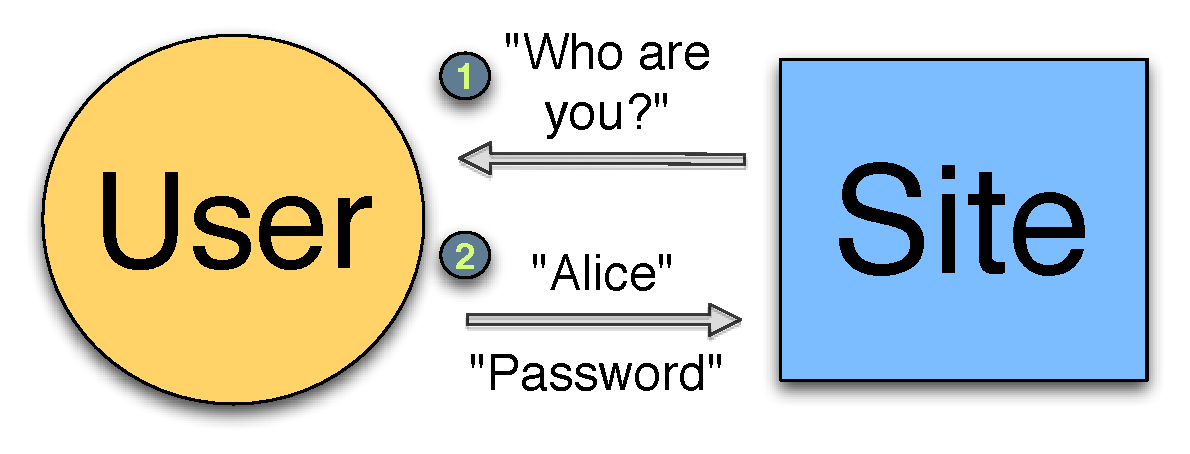
\includegraphics[scale=0.4]{figs/fig-passwd-color.pdf}
  \caption{A user logs in to a website.}
  \label{fig:passwd}
\end{figure}

\begin{itemize}
 \item<1-> Very inconvenient for users
 \item<2-> Insecure workarounds: writing down or reusing passwords
\end{itemize}

\end{frame}

\subsection{Federated Login}

\begin{frame}{New Login Flow}
  \begin{columns}[T]
    \begin{column}{6cm}
      \begin{figure}
         \centering
         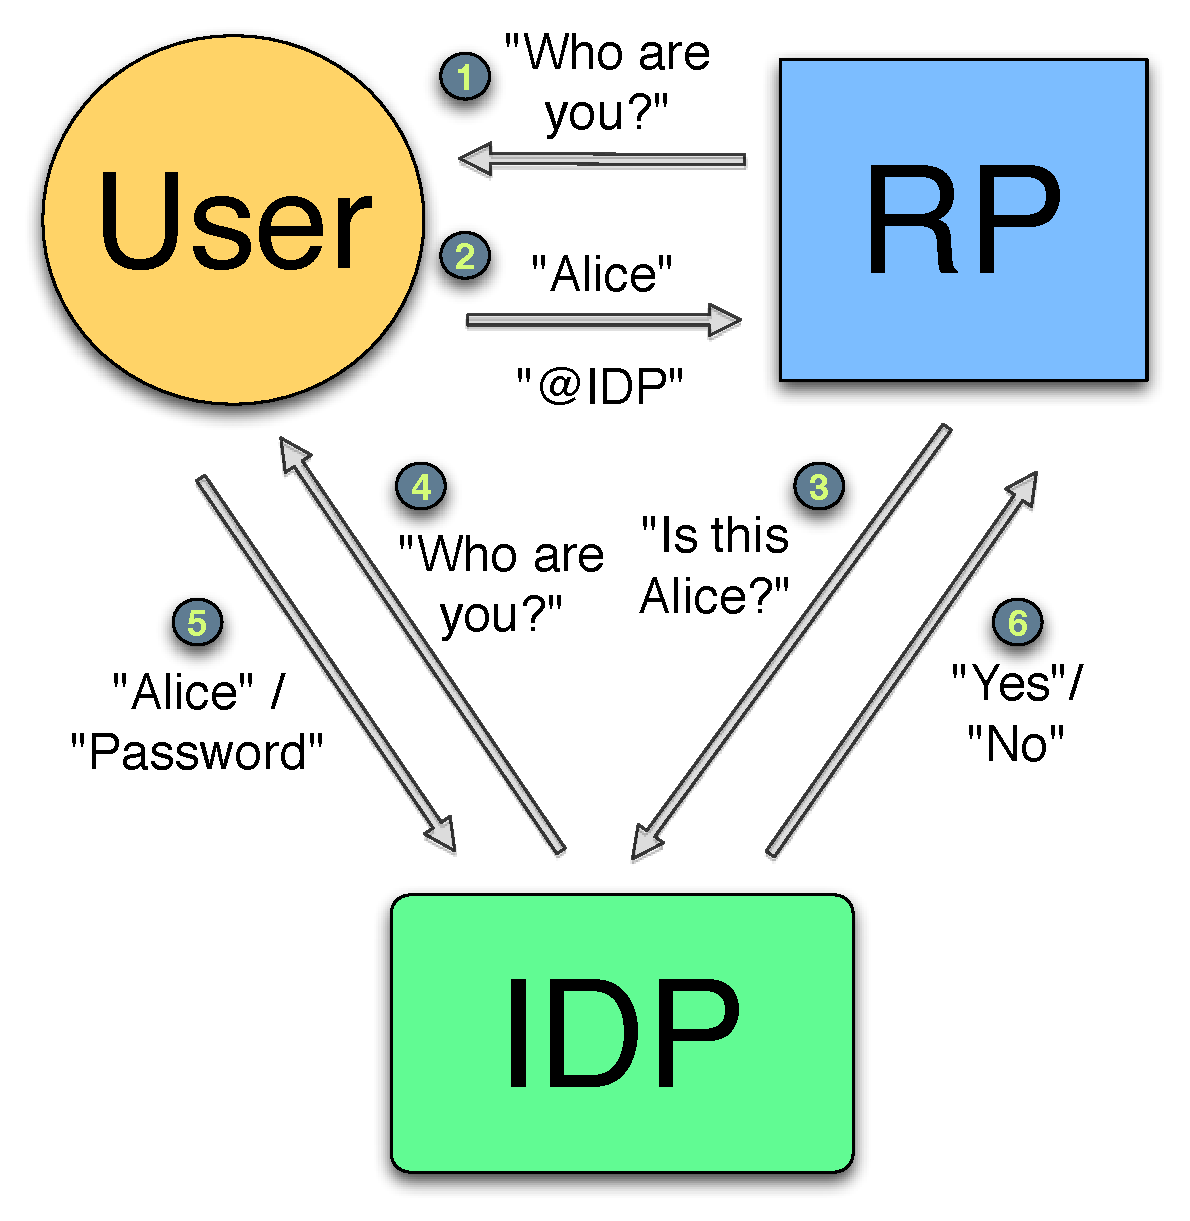
\includegraphics[scale=0.3]{figs/fig-fedlog-color.pdf}
%        \caption{OpenID, a federated login system: the relying party (RP) redirects
%        the user to her identity provider (IDP) for authentication.}
%        \label{fig:fedlog}
      \end{figure}
    \end{column}
    \begin{column}{5cm}
      \begin{enumerate}
        \item RP asks user to authenticate
	\item User supplies IDP name
	\item RP asks IDP to verify user
	\item IDP asks user to authenticate
	\item User authenticates to IDP
	\item IDP asserts user's validity to RP
      \end{enumerate}
    \end{column}
  \end{columns}
\end{frame}

\begin{frame}{Identity Provider Pros and Cons}
  \begin{columns}[t]
    \begin{column}{5cm}
      {\LARGE{Benefits}}
        \begin{itemize}
          \item<1-> Authentication as a service
          \item<2-> Allows Single Sign-On
          \item<3-> Centralized aggregation of user attributes
        \end{itemize}
    \end{column}
    \begin{column}{5cm}
      \uncover<4->{{\LARGE{Privacy Concerns}}}
        \begin{itemize}
          \item<4-> IDP can track its users
          \item<5-> Log destruction often not an option
          \item<6-> Log anonymization difficult (e.g. AOL, Netflix)
        \end{itemize}
    \end{column}
  \end{columns}
\end{frame}

\section{The Solution}

\begin{frame}{Overview of PseudoID}
  \begin{itemize}
    \item Adds a new party: blind signature service (BSS)
    \item Two-phase login
      \begin{itemize}
        \item Setup Phase with BSS: one-time, get access token (AT)
        \item Signon Phase with IDP: use access token
      \end{itemize}
  \end{itemize}
\end{frame}

\subsection{Blind Signature Service}

\begin{frame}{Blind Signatures}

\begin{definition}[Digital Signatures]
A \emph{signer} has a private signing function $\sigma$ which produces
signatures $(m, \sigma(m))$ on a message $m$. There is a public verifier
predicate $V$ such that $V(m, \sigma(m))$ is true iff $m$ has been signed by the
signer.
\end{definition}


\begin{definition}[Blind Signature Schemes]
The provider of a message $m$ uses an pair of \emph{blinding} and
\emph{unblinding} functions $(B,B^{-1})$ that only he knows. The functions
satisfy $B^{-1}(\sigma(B(m))) = \sigma(m).$
\end{definition}

\end{frame}

\begin{frame}{How Blind Signatures Work}

\begin{alertblock}{Blind Signature Protocol}
  \begin{enumerate}
    \item<1-> Generate a message $m$.
    \item<2-> Generate a pair of blinding and unblinding functions $(B,B^{-1})$.
    \item<3-> Blind the message $B(m)$.
    \item<4-> Send the blinded message to the blind signer.
    \item<5-> Receive a signature on the blinded message $\sigma(B(m))$.
    \item<6-> Unblind the signature to receive a signature $\sigma(m)$.
  \end{enumerate}
\end{alertblock}

\end{frame}

\begin{frame}{Blind Signer Setup}
  \begin{figure}
    \centering
    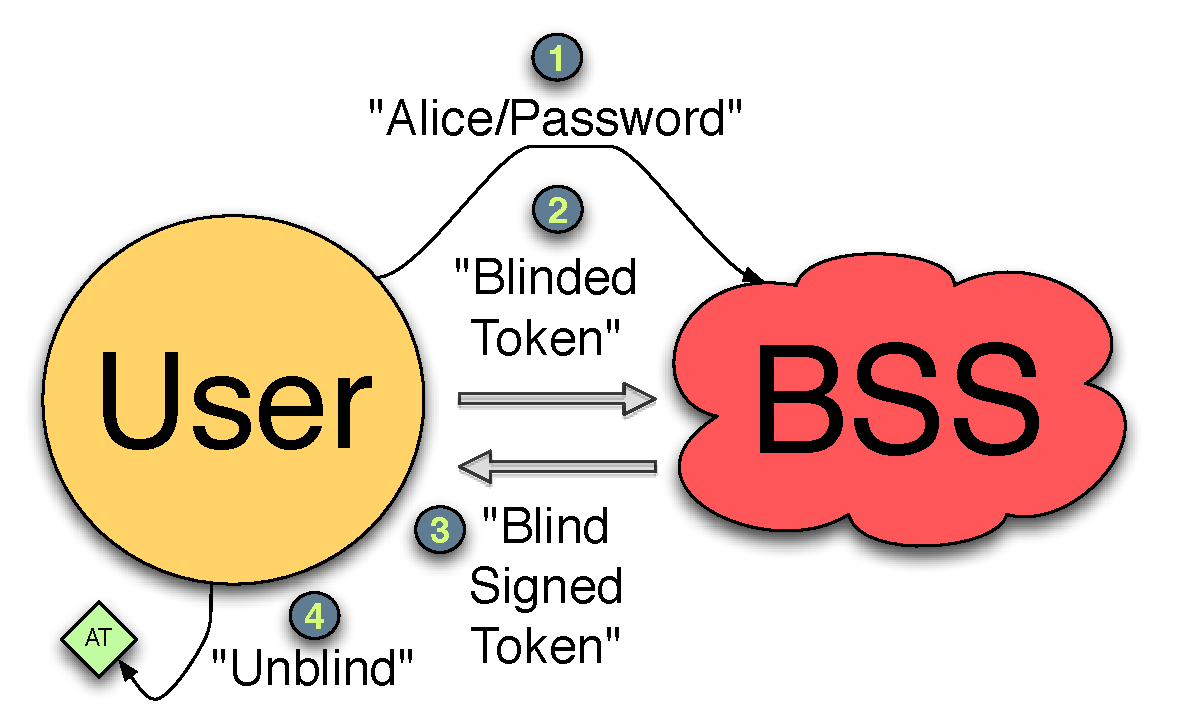
\includegraphics[scale=0.5]{figs/fig-bss-setup-color.pdf}
  \end{figure}
\end{frame}

\begin{frame}{Blind Signer Setup Steps}
  \begin{alertblock}{Blind Signer Setup Protocol}
    \begin{enumerate}
      \item<1-> User authenticates normally.
      \item<2-> User sends BSS a blind token to sign.
      \item<3-> BSS signs token and returns it.
      \item<4-> User unblinds the blind signed token, gets valid, untraceable
access token (AT).
    \end{enumerate}
  \end{alertblock}
\end{frame}

\subsection{Private Identity Provider}

\begin{frame}{Objectives for a Private IDP}
  \begin{itemize}
    \item<1-> Persistent ownable pseudonym
    \item<2-> Pseudonym unlinkable with real identity
    \item<3-> Allow for \emph{selective disclosure} of user attributes
  \end{itemize}

  \begin{example}<4->[Selective Disclosure of Age]
    Website needs to know if you are over 21. Instead of giving them your entire
    birthdate, you present them a signed assertion that you are over 21.
  \end{example}
\end{frame}

\begin{frame}{Complex Identities}
  \begin{itemize}
    \item<1-> A \emph{real} identity is tied with real attributes, more value to
    interaction with application.
    \item<2-> An \emph{imaginary} identity has fake attributes, more privacy.
    \item<3-> Many existing solutions allow you to have a purely real or a
    purely imaginary identity.
    \item<4-> PseudoID gives you \emph{complex} identity, ability to attest your
    real attributes, while maintaining privacy.
  \end{itemize}
\end{frame}

\begin{frame}{The Private IDP Signon Process}
  \begin{figure}
    \centering
    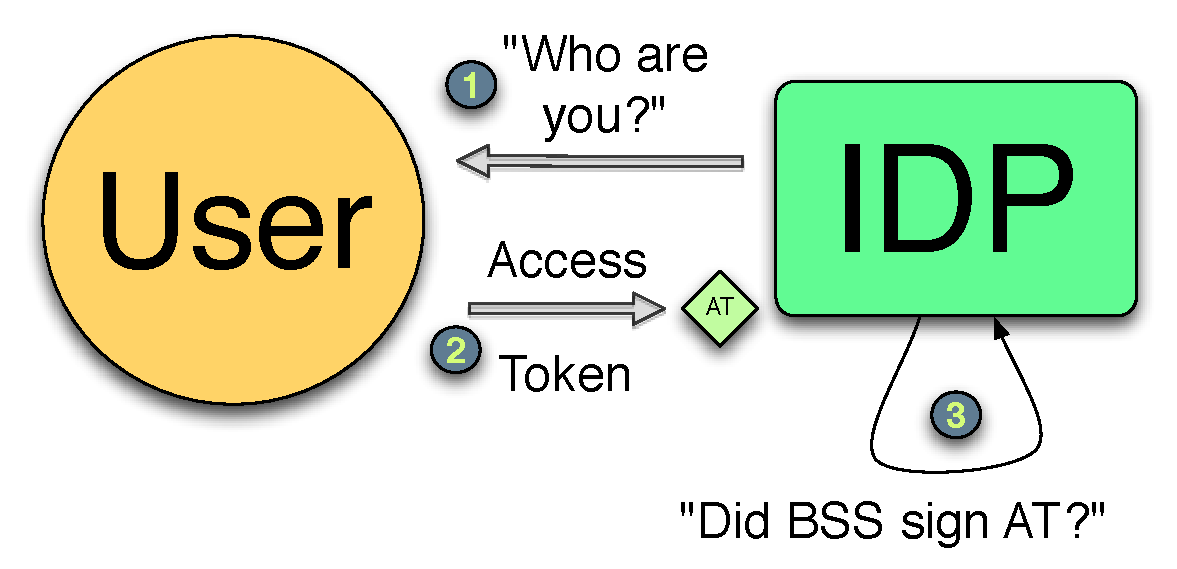
\includegraphics[scale=0.5]{figs/fig-bss-signon-color.pdf}
  \end{figure}
\end{frame}

\begin{frame}{OpenID Integration}

\begin{itemize}
  \item<1-> PseudoID is backwards-compatible with OpenID
  \item<2-> RPs do not have to change at all
  \item<3-> RPs cannot distinguish private IDPs from regular IDPs
\end{itemize}

\begin{alertblock}<4->{DEMO}
PseudoID Demo with access tokens stored in cookies.
\end{alertblock}
\end{frame}

\section[Technical Issues]{Technical Issues and Browser Limitations}

\subsection{Access Tokens}

\begin{frame}{Storing Tokens}
  \begin{itemize}
    \item<1-> Browser lacks persistent storage
    \item<2-> Using client applications/plugins (e.g. Gears) bad for adoptability
    \item<3-> Stored tokens in cookies
    \item<4-> Cookies are very ephemeral, hard to synchronize across computers
  \end{itemize}
\end{frame}

\begin{frame}{Sending Tokens}
  \begin{itemize}
    \item<1-> Tokens created by JavaScript on BSS domain
    \item<2-> Tokens need to be readable by private IDP but not BSS
  \end{itemize}

  \begin{definition}<3->[Same-Origin Policy]
    Two pages have the \emph{same origin} if they have same protocol, port, and
    host.
  \end{definition}

  \begin{itemize}
    \item<4-> BSS cannot set cookie on IDP's domain
    \item<5-> BSS cannot make an AJAX call to IDP
  \end{itemize}
\end{frame}

\begin{frame}{Cooperative Cross-Domain Communication}
  \begin{itemize}
    \item<1-> Can source external scripts, images, stylesheets, iframes
    \item<2-> Can pass messages in URL query string or fragment identifier
  \end{itemize}

  \begin{alertblock}<3->{Cross-Domain Cookies with Iframes}
    JavaScript on BSS loads a \emph{hidden iframe} to an IDP service and passes
    cookie in the fragment identifier. IDP retrieves cookie from the fragment
    and sets it on its own domain.
  \end{alertblock}
\end{frame}

\begin{frame}{Need Better Browser Capabilities}
  \begin{itemize}
    \item<1-> Applications already implementing one-off hacks
    \item<2-> Need a message passing mechanism within the browser
    \item<3-> Domain A can send a message to Domain B through JavaScript API if
    A is on B's whitelist of senders
  \end{itemize}

  \begin{example}<4->[What It Might Look Like]
  Add \texttt{document.send(domain, msg)} and \texttt{document.receive(domain,
  msg)} methods to JavaScript API.
  \end{example}
\end{frame}

\subsection{Side Channels}

\begin{frame}{Traffic Analysis}
  \begin{itemize}
    \item<1-> IDP can still track your IP address.
    \item<2-> Need to use TOR, anonymize IP.
    \item<3-> Attacker can also track user visit times to BSS and IDP.
  \end{itemize}
\end{frame}

\begin{frame}{Other Cookies}
  \begin{itemize}
    \item<1-> Malicious parties can still track user by attaching random cookie.
    \item<2-> Need to scrub other cookies from BSS after obtaining access token.
    \item<3-> May want to just not store any cookies for BSS.
  \end{itemize}
\end{frame}

\begin{frame}{Untrusted Javascript}
  \begin{itemize}
    \item<1-> Security relies on the proper blinding and unblinding of token
    \item<2-> Blinding/Unblinding done in JavaScript
    \item<3-> Need to serve script from a trusted source.
    \item<4-> Malicious script may redefine JavaScript keywords, skip blinding
    steps, phone home, etc...
  \end{itemize}
\end{frame}

\section*{Summary}

\begin{frame}{Summary}
  \begin{itemize}
    \item<1-> Federated login adds convenience at expense of user privacy.
    \item<2-> Private identity providers using a blind signer can give users
    untraceable pseudonyms.
    \item<3-> Blind signer allows IDPs to support \emph{selective disclosure} of
    attributes.
    \item<4-> Need more robust browser storage and better cross-domain
    communication.
  \end{itemize}
\end{frame}

\end{document}
